%!TEX root = ../abgabe.tex

\section{Beispiel}

Geschrieben von: \textbf{Hans-Thorben Juilfs}
\newline

In dieser Sektion geht es um ein Fallbeispiel. Das Re-Design und die Entstehung dessen werden beleuchtet und erklärt. Außerdem wird im Folgenden auf einzelne, wichtige Komponenten in der Planung des Designs, sowie der Vorgehensweise eingegangen. Zunächst wird es um die UI-Komponenten(User Interface) gehen.\\

Das Fallbeispiel ist das Re-Design von der iOS app ''AutoTrader'' für Android. Wir haben uns entschieden die im Referat vorgestellte Navigationssoftware nicht noch einmal zu beschreiben, sondern auf eine etwas aktuellere Software zurückzugreifen, um neuere Designaspekte deutlicher ausleuchten zu können.

Dabei werden einige Beispiele aufgeführt, die bebildert beschrieben werden und so den Zugang erleichtern.\\

Die vorliegenden Informationen beruhen auf dem Buch ''Android Design Patterns: Interaction Design Solutions for Developers'' von Greg Nudelman\\


\subsection{Logo-Design}
\label{sub:logodesign}
Zunächst wird das Logo und das ensprechende Re-Design beschrieben:\\

\begin{figure}[h]
 \centering
 
\includegraphics[height=0.10\textheight]{img/logo.png}
 \caption{Re-Design des Logos}
\end{figure}

Ein Logo wird nach Vorschrift von Apple Inc. immer viereckig, mit abgerundeten Ecken dargestellt. Diese Limitation liegt für Android app-logos nicht vor. Hier wird mehr künstlerische Freiheit gegeben. Um dies zu verdeutlichen wird -einfach ein Teil des iOS app-logos genommen und als neues Logo angepasst.\cite{AndroidDesignPatterns}


\subparagraph{Vorher}
\label{subp:vorher}
Ersteinmal beschreibt der Autor Greg Nudelman das Aussehen der App bevor das Design angepasst wurde. Hierbei wird aufgezeigt, dass ein großer Knopf mit der Aufschrift ''Settings'' nichts an dem angestammten Platz in der oberen rechten Ecke des Bildschirmes zu suchen hat, da es sich dabei um eine der wichtiges Positionen auf der GUI handelt. Hinzukommt, dass der Knopf keine Einstellungen zeigt, wenn er ausgelöst wurde, sondern lediglich eine ''Anwalts''-Seite zeigt, auf der sich ''Privacy Policy'', ''Visitor Agreement'' und ein Knopf mit der Aufschrift ''Email-Feedback'' befinden.\cite{AndroidDesignPatterns}\\

\begin{figure}[h]
 \centering
 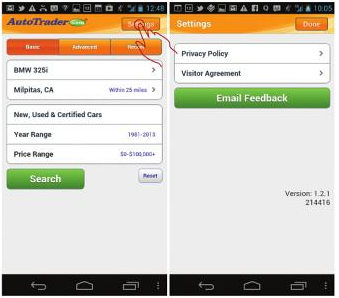
\includegraphics[height=0.40\textheight]{img/Design1.png}
 \caption{Re-Design des Logos}
\end{figure}

Da der ''Settings''-Knopf so einen wichtigen Platz einnimmt, werden wichtigere Funktionen, wie ''Find cars'', ''Find dealer'' oder ''Scan \& Find'' in den Hintegrund gedrängt und sind in einer einem älteren Android nachempfundenen navigation bar menu versteckt.

\begin{figure}[h]
 \centering
 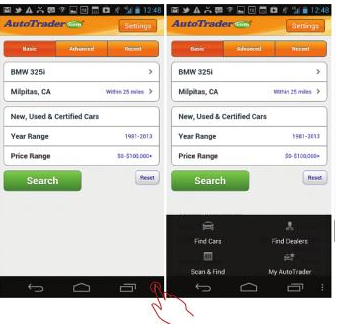
\includegraphics[height=0.40\textheight]{img/Design2.png}
 \caption{Re-Design des Logos}
\end{figure}

\subparagraph{Nachher}
\label{subp:nachher}


\subsection{Beispiele}
\label{sub:examples}

\subparagraph{Home Screen}
\label{subp:home_screen}

\subparagraph{Routenplaner}
\label{subp:route_planner}

\subparagraph{Karten}
\label{subp:maps}

\subparagraph{Verkehr}
\label{subp:traffic}

\subparagraph{Icons}
\label{subp:icons}

\subparagraph{Interaktion}
\label{subp:interaction2}

\subsection{Resultate des Projektes} 
\label{sub:results_of_the_project}

\subparagraph{Lessons learned}
\label{subp:lessons_learned}

\subparagraph{Projekt Dokumentaion}
\label{subp:documentation}

\subparagraph{Vergleich mit anderes Systemen}
\label{subp:comparison_to_other_systems}